\chapter{Cifrari Simmetrici}
Un cifrario simmetrico è composto principalmente da tre cose:
\begin{itemize}
    \item \textbf{KeyGen:} Algoritmo randomizzato di generazione di una chiave da un insieme $K$.
    \item \textbf{Enc:} Algoritmo di Encryption a stati o randomizzato che prende in input una chiave k e un messaggio m e restituisce un crittotesto C. 
    \item \textbf{Dec:} Algoritmo deterministico in grado di ritornare al messaggio m a partire da (k,C).
\end{itemize}

Un cifrario simmetrico è \textbf{randomizzato} se utilizza una qualche quantità di randomness. Diciamo, invece, che un cifrario è a stati se il risultato dipende da una certa quantità detta \textbf{stato}. Questi cifrari utilizzano meccanismi di cifratura a blocchi e, per semplicità, supporremo che la dimensione del messaggio è un multiplo della taglia del blocco.
\section{Modo ECB (Electronic Codebook Mode)}
Sia $E:K\times \{0,1\}^n \xrightarrow{} \{0,1\}^n$ un cifrario a blocchi, ECB produce un cifrario senza stati e deterministico. L'algoritmo di generazione della chiave si limita a restituire una stringa random e, per effettuare Encryption e Decryption utilizziamo i seguenti algoritmi:
\begin{figure}[H]
    \centering
    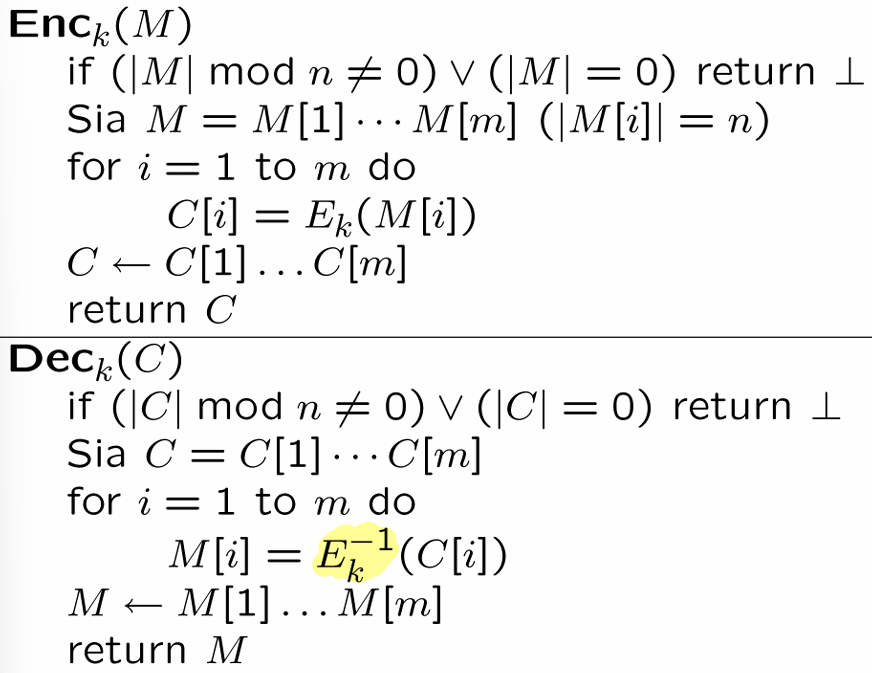
\includegraphics[width=0.5\linewidth]{Images/cifrari_simmetrici/modo_ecb_deterministico.png}
\end{figure}

Questo algoritmo non fa altro che dividere il messaggio in vari blocchi ed effettuare encryption blocco per blocco in base a una chiave scelta a random. Allo stesso modo, a partire dalla chiave, si effettua la decryption del messaggio.


\section{Modo CBC\$ (Cipher block Chaining Mode)}
Questo modo è \textbf{randomizzato} e lo possiamo denotare dalla presenza del \$ nel nome che, d'ora in avanti, indicherà tutti i cifrari randomizzati.
Sia $E:K\times \{0,1\}^n \xrightarrow{} \{0,1\}^n$ un cifrario a blocchi, CBC\$ genera un vettore iniziale random detto \textbf{IV} e, tramite questo, effettua la cifratura del messaggio. In questo caso, la chiave sarà semplicemente una stringa random di una certa lunghezza. Viene, inoltre, definito \textbf{Chain model} perché una singola decisione, cambia tutta la catena di cifratura. \footnote{In questo caso la decisione è il vettore iniziale IV}
\begin{figure}[H]
    \centering
    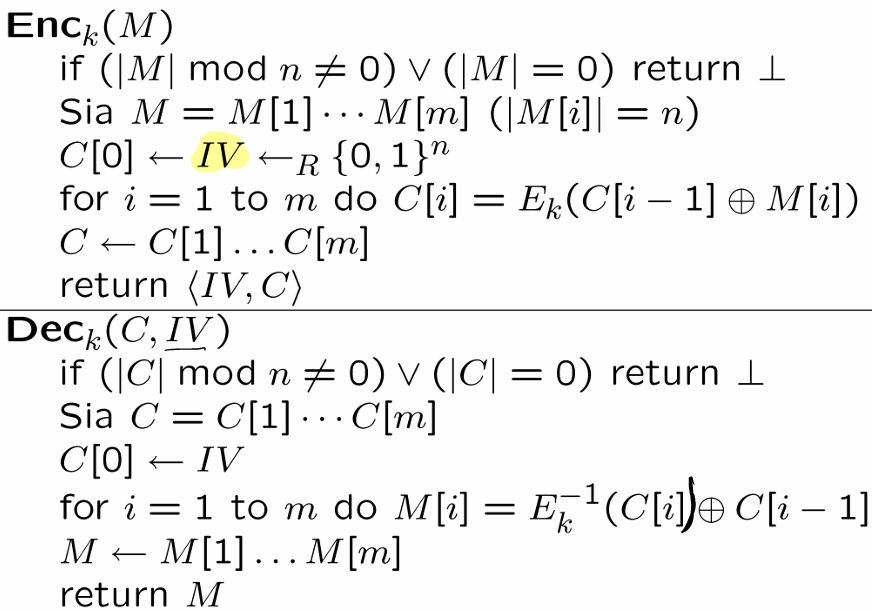
\includegraphics[width=0.5\linewidth]{Images/cifrari_simmetrici/modo_cbc_random.png}
\end{figure}

Anche in questo caso l'algoritmo divide il tutto in blocchi, dopodiché, imposta una cifratura a catena con $C[0]=IV$ e, i successivi blocchi $C[i]$ saranno $C[i] = E_k (C[i-1] \oplus M[i])$. Come possiamo notare, è necessario ritornare anche il vettore IV per poter effettuare la decifratura. Per decifrare il tutto faremo l'operazione inversa sempre a partire dello stesso $C[0]$ poiché $M[i] = C[i-1] \oplus E_k^{-1}(C[i])$.
\section{Modo CTR\$ (counter randomizzato)}
Sia $F:K\times \{0,1\}^l \xrightarrow{} \{0,1\}^L$ una famiglia di funzioni, CTR\$ produce un cifrario randomizzato senza stati. Anche in questo caso, la chiave sarà semplicemente una stringa random. E, una precisazione necessaria da fare è che in questo specifico modo non abbiamo la necessità che la dimensione del messaggio sia multiplo del blocco. 

\begin{figure}[H]
    \centering
    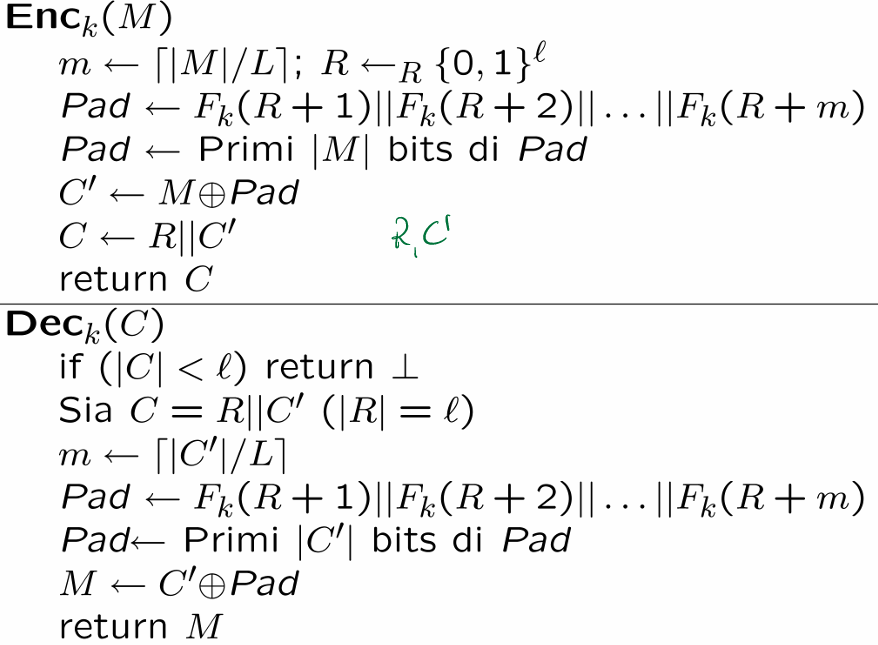
\includegraphics[width=0.5\linewidth]{Images/cifrari_simmetrici/modo_ctr_random.png}
\end{figure}

Quello che facciamo è dividere anche in questo caso il messaggio in "blocchi" e, successivamente, generiamo $Pad = F_k(R+1)||F_k(R+2)||\dots||F_k(R+m)$ dove R è una stringa random che funge da componente random\footnote{NB: Ricordiamo che R è diverso dalla chiave}. Una volta generato il pading, prendiamo solo i bit che ci servono e facciamo uno xor tra il messaggio M e Pad. Anche in questo caso, come prima, abbiamo la necessità di salvare in qualche modo la chiave R che, semplicemente, concateniamo al crittotesto. Per quanto riguarda la decryption, generiamo nuovamente il pading e rifacciamo lo xor con il crittotesto, ottenendo nuovamente il messaggio.

\section{Modo CTRC (modo counter non randomizzato)}
Questo modo non è altro che CTR\$ che, invece di essere randomizzato è a \textbf{stati}. In pratica, teniamo un contatore globale ctr, inizialmente a 0, che utilizziamo allo stesso modo di come utilizzavamo prima la componente random. 
\begin{figure}[H]
    \centering
    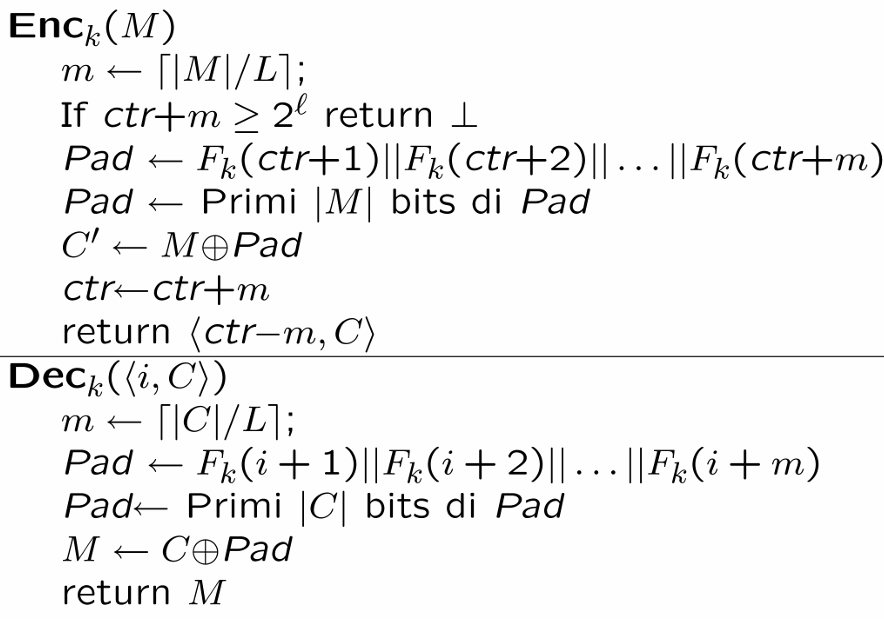
\includegraphics[width=0.5\linewidth]{Images/cifrari_simmetrici/modo_ctr_stati.png}
\end{figure}

\section{Privacy}
Come facciamo, adesso visti alcuni esempi, a scegliere quale cifrario utilizzare e quale è il migliore rispetto a un altro cifrario. Il nostro obiettivo sarà quelli di definire in maniera soddisfacente la sicurezza o cosa rappresenta la privacy di un sistema di questo tipo così da poter stabilire un metodo di confronto tra i vari modi.

Chiaramente a primo impatto una definizione che sembra funzionare è che se A può dedurre M da C, allora lo schema non è sicuro. Tuttavia, questa cosa non funziona ugualmente poiché anche alcune informazioni parziali potrebbero fare la differenza. Abbiamo, dunque, bisogno di una definizione più forte esattamente come abbiamo fatto per i cifrari a blocchi.

Idealmente vorremmo che il nostro testo cifrato non riveli alcuna informazione riguardo al messaggio M, tuttavia alcune informazioni a priori sono inevitabili da mostrare come, ad esempio, la dimensione del messaggio poiché non possiamo comprimere il messaggio più di una certa dimensione e non possiamo allungare il messaggio più di tanto perché rischieremmo di floodare la rete. Tuttavia, analizzando ECB può giungerci un suggerimento. 
Come abbiamo visto ECB è un cifrario del tutto deterministico, per cui, cifrando due blocchi esattamente uguali, vedremo esattamente lo stesso risultato. Ergo, la proprietà che sceglieremo sarà proprio quella di \textbf{indistinguibilità} rispetto ad attacchi a \textbf{testo scelto}. 

\section{Indistinguibilità}
Immaginiamo il seguente esperimento: l'attaccante sceglie una coppia $M_0,M_1$ che manderà ad un oracolo che sceglierà se cifrare solo il $M_0$ o solo $M_1$. L'obiettivo dell'attaccante sarà quello di riuscire a capire quale dei due messaggi è stato cifrato a patto che $|M_0| = |M_1|$. L'attaccante potrà fare più domande anche basate sulle risposte precedenti sempre a patto che le domande siano computazionalmente fattibili.
\begin{figure}[H]
    \centering
    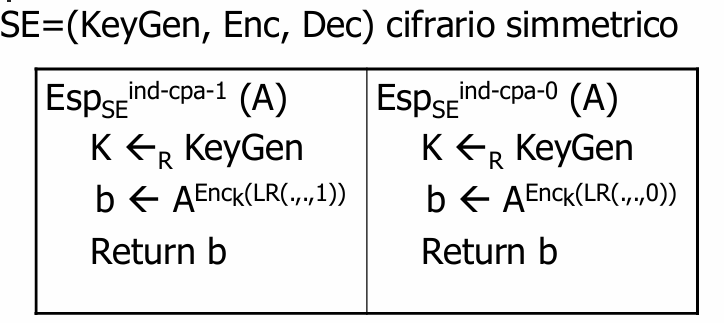
\includegraphics[width=0.5\linewidth]{Images/cifrari_simmetrici/esperimento_indistinguibilita.png}
\end{figure}

Anche in questo caso possiamo definire il vantaggio dell'attaccante A come:
\[Adv^{ind-cpa}(A)=|Pr[Esp_{SE}^{ind-cpa-1}(A)=1]-Pr[Esp_{SE}^{ind-cpa-0}(A)=1]|\]

Se l'avversario può vincere con probabilità $1/2$ questo non è considerabile una minaccia poiché equivarrebbe al tentare a casaccio. Il vantaggio più sarà prossimo a 1 più l'attaccante avrà probabilità di dare la risposta corretta. 

Equivalentemente all'esperimento precedente, possiamo scrivere:
\begin{figure}[H]
    \centering
    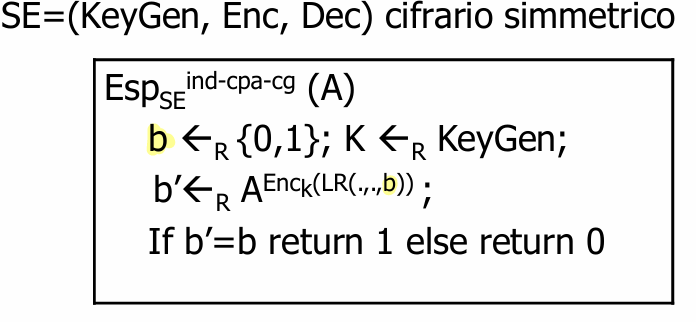
\includegraphics[width=0.5\linewidth]{Images/cifrari_simmetrici/esperimento_indistinguibiltita_alternativo.png}
\end{figure}
E in questo caso il vantaggio cambierebbe in:\footnote{Si può dimostrare e la dimostrazione è presente nelle slide}
\[Adv^{ind-cpa}(A)=2Pr[Esp_{SE}^{ind-cpa-cg}(A)=1]-1\]

Tornando a ECB, ci possiamo facilmente rendere conto come fallisca in questo specifico esperimento poiché possiamo costruire un'attaccante in grado di rispondere con certezza quale dei due messaggi è stato cifrato:
\begin{figure}[H]
    \centering
    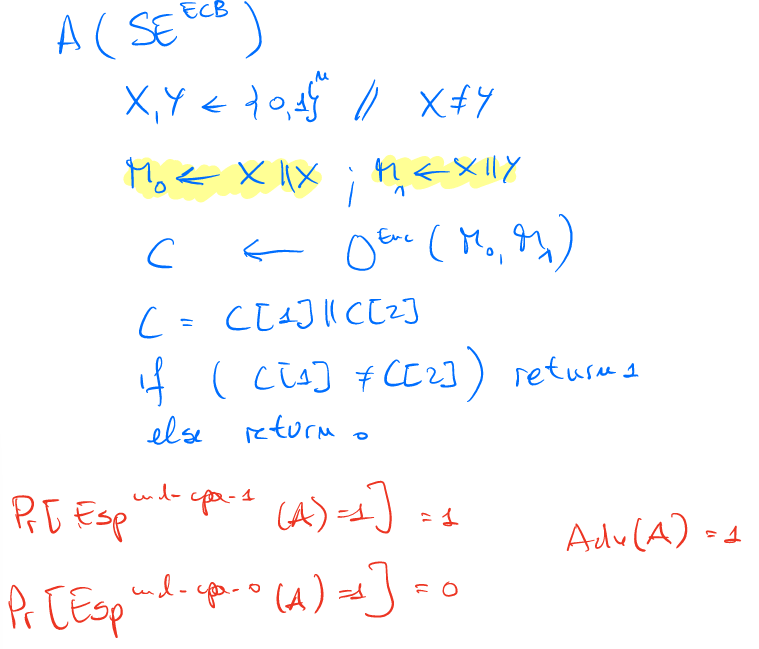
\includegraphics[width=0.5\textwidth]{Images/cifrari_simmetrici/attaccante_ecb.png}
\end{figure}

Da qui possiamo notare come, in realtà, qualunque schema di cifratura deterministico e senza stati sia del tutto insicuro. Proviamo adesso a dimostrare che se un eventuale attacco di plain text recovery funziona, allora rompe lo schema anche in senso di indistinguibilità.
Partiamo semplicemente da un cifrario simmetrico senza stati e facciamo il seguente esperimento:
\begin{figure}[H]
    \centering
    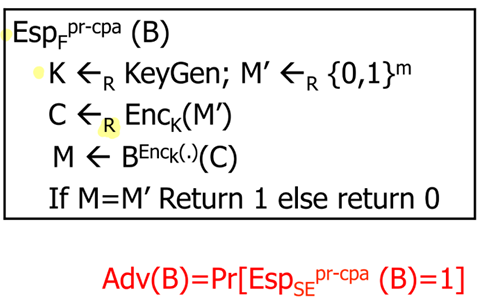
\includegraphics[width=0.5\linewidth]{Images/cifrari_simmetrici/esperimento_pr_cpa_b.png}
\end{figure}

Per cui, l'obiettivo di B sarà quello di indovinare il testo del messaggio cifrato a partire dalla sua cifratura potendo fare domande del tipo a questo input quale output corrisponde. Il suo vantaggio sarà in questo caso:
\[Adv(B)=Pr[Esp_{SE}^{pr-cpa}(B)=1]\]
Ragionando su questo vantaggio, dobbiamo tenere conto del fatto che esiste un numero limitato di messaggi che si possono generare. Per cui, diremo che un buon vantaggio deve sicuramente essere maggiore di $\frac{1}{2^m}$. L'attacco quindi sarà banalmente il seguente: 
\begin{figure}[H]
    \centering
    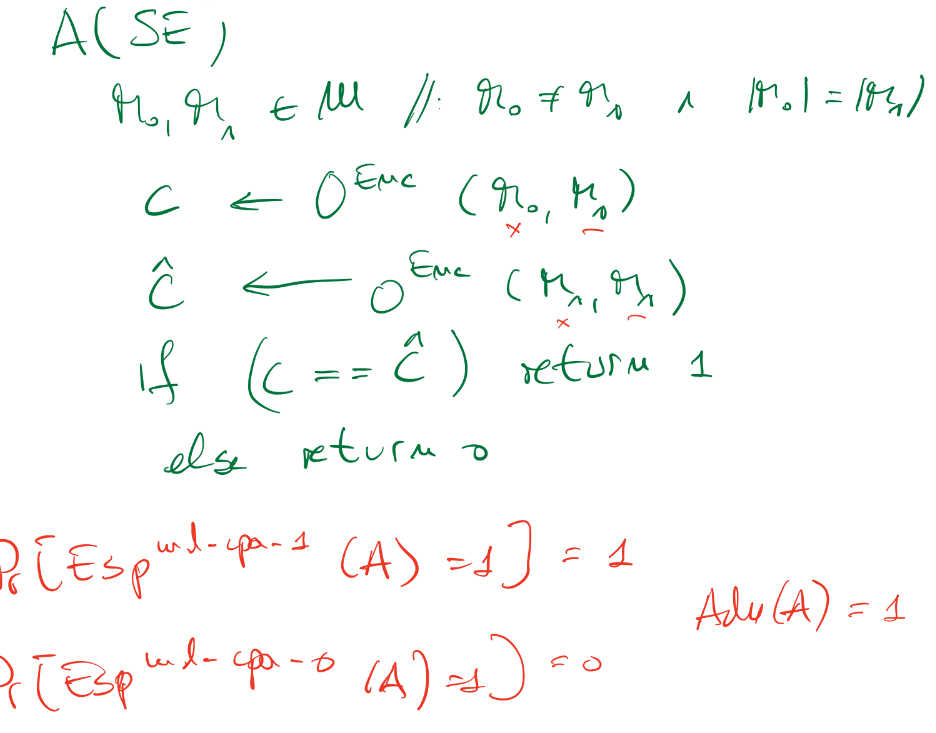
\includegraphics[width=0.5\linewidth]{Images/cifrari_simmetrici/attacco_deterministico.png}
\end{figure}

Come abbiamo fatto per la pseudo casualità, possiamo costruire un attaccante A che attacca il cifrario nel senso di indistinguibilità, sfruttando anche B, per cui varrà che:
\[Adv(B)\leq Adv(A)+\frac{1}{2^m}\]
\begin{figure}[H]
    \centering
    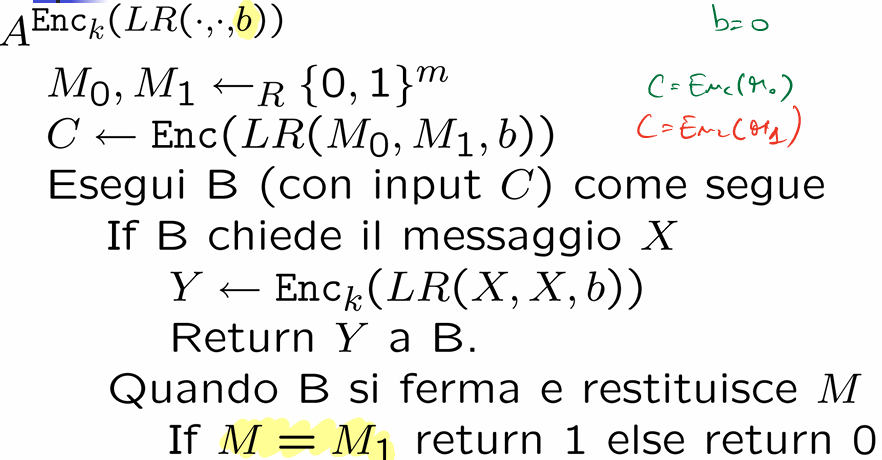
\includegraphics[width=0.5\linewidth]{Images/cifrari_simmetrici/esperimento_ind_cpa_A.png}
\end{figure}
Avremo che B quando chiede l'encryption di un messaggio passerà in input due volte la stessa stringa poiché l'oracolo è del tipo che cifra o solo il messaggio a sinistra o solo il messaggio a destra. 
Secondo questa definizione dell'attaccante A, avremo che:
\begin{align*}
    &Pr[Esp^{ind-cpa-1}(A)=1] = Adv(B)\\
    &Pr[Esp^{ind-cpa-0}(A)=1] = \frac{1}{2^m}
\end{align*}

Un'ulteriore generalizzazione dell'indistinguibilità si può ottenere considerando un qualunque predicato e mostrando che, se si può estrarre, allora questo cifrario non è indistinguibile. Ragioniamo esattamente come prima, definiamo innanzitutto l'esperimento di B:
\begin{figure}[H]
    \centering
    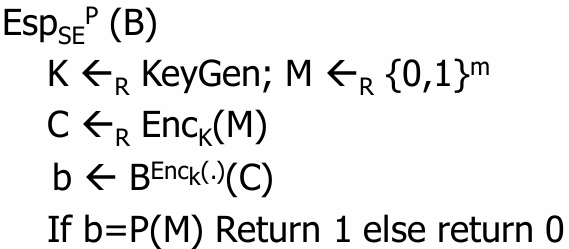
\includegraphics[width=0.5\linewidth]{Images/cifrari_simmetrici/esperimento_predicato_B.png}
\end{figure}
Il vantaggio di B sarà in questo caso $2Pr[Esp_{SE}^P(B)=1]-1$.
Per cui creiamo un attaccante A che sfrutta B tale che il vantaggio di A sia:
\[Adv(B)=Adv(A)\]
\begin{figure}[H]
    \centering
    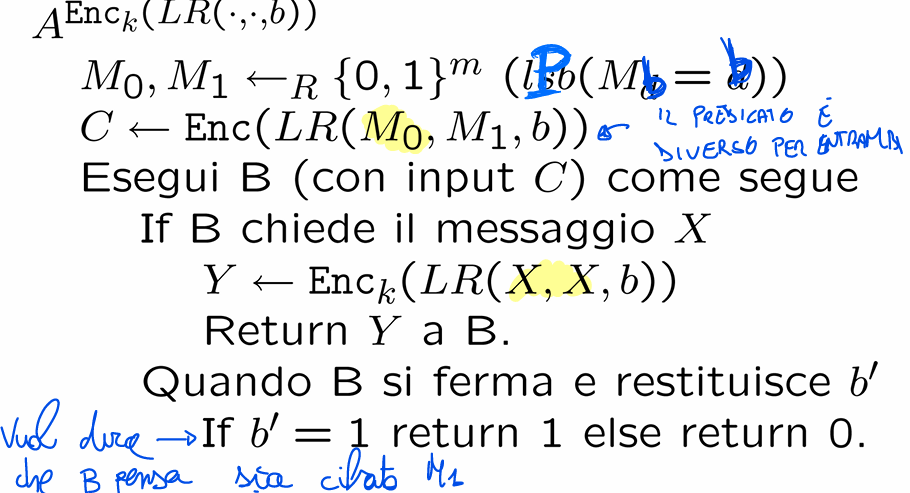
\includegraphics[width=0.5\linewidth]{Images/cifrari_simmetrici/esperimento_predicato_A.png}
\end{figure}
Come segnato, l'attaccante A sceglie random due messaggi per cui il predicato per ognuno ha un valore diverso.\footnote{Essendo un predicato il valore sarà o 0 o 1 e $P(M_1)=1$ e $P(M_2)=2$} Dopodiché verrà eseguito B e darà la sua risposta cercando di capire se è stato cifrato il messaggio 0 o 1 in base al predicato che lui pensa possa avere quel testo cifrato mandato in input. Se B ritorna 1 vuol dire che pensa sia stato cifrato il messaggio 1 e che, quindi, il testo cifrato in input avesse il predicato 1, altrimenti si ragiona in modo speculare per il messaggio 0.

Cerchiamo di capire se il vantaggio è uguale:
\begin{align*}
    &Pr[Esp^{ind-cpa-1}(A)=1] = Pr[B\xrightarrow{}1] \\
    &= Pr[\text{B indovina P($M_1$)}] = Pr[Esp^p(B)=1]\\
    \\
    &Pr[Esp^{ind-cpa-0}(A)=1] = Pr[b'=1] = Pr[B\xrightarrow{}1]\\
    &=Pr[B\text{ non indovina P($M_0$)}] = 1-Pr[\text{B indovina P($M_0$)}]=\\
    &= 1-Pr[Esp^p(B)=1]
\end{align*} 

Poiché abbiamo che: 
\[Adv^{ind-cpa}(A) = |Pr[Esp^{ind-cpa-1}(A)=1] - Pr[Esp^{ind-cpa-0}(A)=1]|\] 
utilizzando questa formula avremo che:
\[Pr[Esp^p(B)=1]-(1-Pr[Esp^p(B)=1])=2Pr[Esp^p(B)=1]-1\]
Che è esattamente il vantaggio di B. Questo esperimento ci mostra che se non possiamo estrarre un predicato generico dal cifrario, allora non possiamo neanche attaccare il cifrario per indistinguibilità.

\section{Sicurezza di CTRC e CTRC\$}
Adesso che abbiamo dimostrato tutto ciò, possiamo dimostrare che i modi CTR sono sicuri. Per fare un breve ripasso, riguardiamo i due modi di fare encryption:
\begin{figure}[H]
    \centering
    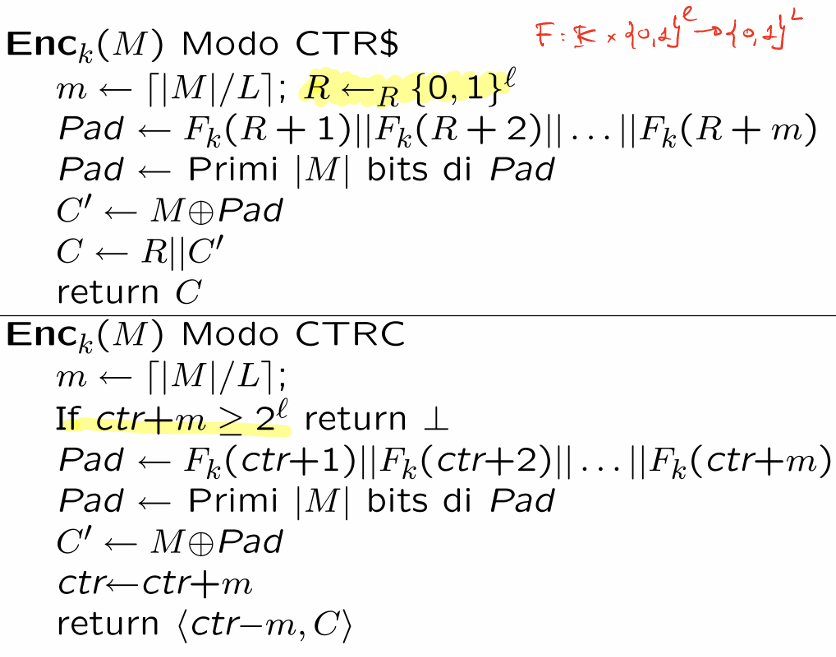
\includegraphics[width=0.7\linewidth]{Images/cifrari_simmetrici/ctrc_ctrrandom.png}
\end{figure}
Nonostante ci aspettiamo che i vantaggi siano uguali, questo non è propriamente vero. La differenza sta nel fatto che in CTR\$ prendiamo delle scelte random e, di conseguenza, siamo soggetti a un attacco basato su paradosso del compleanno mentre, invece, in CTRC ciò non accade perché non abbiamo il rischio di prendere una chiave uguale a una precedentemente scelta.
La dimostrazione che faremo riguarderà solo CTRC. Se prendiamo A un avversario che attacca il cifrario per indistinguibilità facendo q domande per un totale di $\sigma$ blocchi cifrati, esiste un avversario B che fa un attacco contro la sicurezza della PRF che fa $\sigma$ domande e tale che:
\[Adv_{SE}^{ind-cpa}(A) \leq 2Adv_F^{prf}(B)\]

\begin{figure}[H]
    \centering
    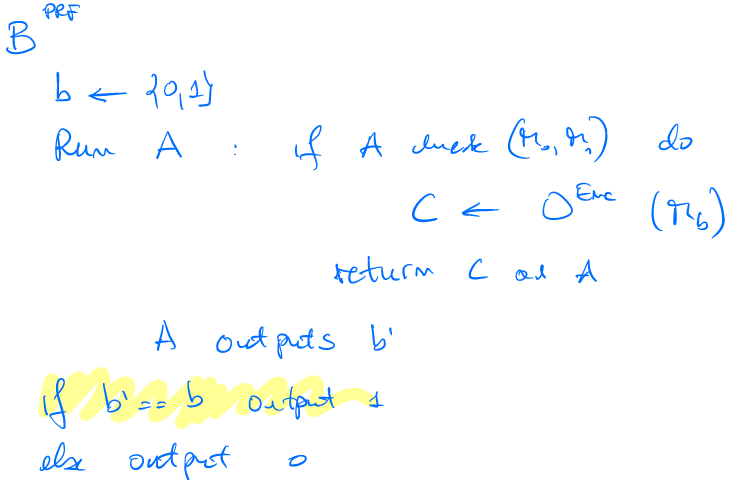
\includegraphics[width=0.7\linewidth]{Images/cifrari_simmetrici/attaccante_B_prf.png}
\end{figure}

B sceglie un bit b che indicherà se verrà cifrata la stringa di sinistra o quella di destra facendo sì che B simuli in tutto e per tutto l'oracolo agli occhi di A. Dopodiché viene lanciato A e, se questo riesce ad indovinare quale stringa sta venendo cifrata, allora B risponde 1, altrimenti risponde 0.
\begin{align*}
    &Pr[Esp^{prf-1}(B)=1] = Pr[Esp^{ind-cpa-cg}(A)=1] \quad \text{/B risponde 1 se A risponde 1}\\
    &= \frac{1}{2}+\frac{1}{2}Adv^{ind-cpa}(A) \quad \text{/Deriva dal fatto che $Adv^{ind-cpa}(A)=2Pr[Esp^{ind-cpa-cg}(A)=1]-1$}\\
    \\
    &Pr[Esp^{prf-0}(B)=1] = Pr[Esp^{ind-cpa-cg}(A)=1] = \frac{1}{2}+\frac{1}{2}Adv^{ind-cpa}(A) = \frac{1}{2}\\
    &\text{/$Adv^{ind-cpa}(A)=0$ nel caso in cui siamo in prf-0 poiché la funzione è totalmente casuale} 
\end{align*}
Dato ciò, avremo che:
\[Pr[Esp^{prf-1}(B)=1]-Pr[Esp^{prf-0}(B)=1]=\frac{1}{2}Adv^{ind-cpa}(A)\]
Da cui, segue che:
\[Adv(B)=\frac{1}{2}Adv(A)\]

Tutto questo ci indica che per rompere questo cifrario è necessario che la PRF non sia sicura. Per cui, se la PRF è sicura, allora CTRC è sicuro.

Per quanto riguarda CTR\$ non dimostreremo formalmente la cosa, tuttavia diremo che vale:
\[Adv_{SE}^{ind-cpa}(A) \leq Adv_F^{prf}(B)+ \frac{0.5 \sigma^2}{2^l}\]
Dove $\frac{0.5 \sigma^2}{2^l}$ rappresenta la possibilità di un attacco basato sul paradosso del compleanno che viene introdotto dalla scelta casuale.

Un'importante cosa da tenere in considerazione sono i parametri che scegliamo nei cifrari come possono essere magari la grandezza dei blocchi, la grandezza della chiave ecc. Facciamo un esempio di scelta di questi parametri per quanto riguarda CTR.

Supponiamo di utilizzare:
\begin{align*}
    &F=AES(l=L=128), q = 2^{30}\\
    &\text{Ogni messaggio ha $2^{13}$ bit} \xrightarrow{}2^{36} \text{ blocchi}
\end{align*}
Posso utilizzare CTR\$ per cifrare q messaggi in modo sicuro? Per rispondere a questa domanda possiamo utilizzare l'avversario A che attacca CTR\$ e, dal teorema precedente, costruiamo B che, ricordiamo, attacca la prf del cifrario.\footnote{Nello specifico AES} Assumendo che AES sia sicuro, il vantaggio di B non può essere superiore a $\frac{\sigma^2}{2^{128}}$ cioè ciò che deriva dalla possibilità di un attacco basato sul paradosso del compleanno. Il teorema ci dice che:
\[Adv_{SE}^{ind-cpa}(A)\leq 2 Adv_F^{prf}(B)\leq \frac{\sigma^2}{2^{128}}+{\sigma^2+0.5}{2^{128}}=\frac{0.5 * 2^{72}}{2^128}\leq \frac{1}{2^{55}}\]

Questo ci dice che se cifriamo più di $\sigma= 2^{l/2}$ blocchi con CTR\$, non possiamo più dimostrare alcuna sicurezza. 
\section{Attacchi a crittotesto scelto}
Fino a ora abbiamo considerato solo attacchi CPA, \footnote{Che è l'attacco a testo scelto} ma possiamo considerare un attacco ancora più forte che è quello a crittotesto scelto per cui forniamo all'attaccante un oracolo che può decifrare i messaggi. Se un cifrario è sicuro verso attacchi CCA, allora sarà sicuro anche nei confronti di CPA e sarà una definizione ancora più forte in un certo senso poiché diamo all'attaccante un'arma ben più forte rispetto a quella che già possiede. 
\begin{figure}[H]
    \centering
    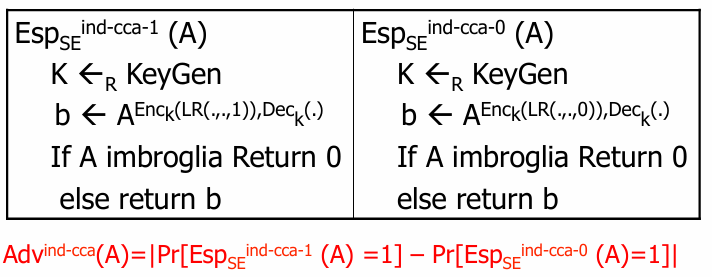
\includegraphics[width=0.7\linewidth]{Images/cifrari_simmetrici/esperimento_cca_1.png}
\end{figure}

In figura possiamo vedere sia l'esperimento considerato che il vantaggio dell'attaccante. Notiamo che se l'attaccante "imbroglia", allora questo ritornerà un valore a caso. Diremo che un'attaccante imbroglia se questo chiede prima la cifratura di due messaggi e poi chiede la decifratura del crittotesto in output.

Proviamo ad attaccare CTR mediante un attacco a crittotesto scelto. Guardiamo il caso CTR\$ e consideriamo il seguente attaccante che sceglierà un messaggio da inviare e lo cifrerà. Dopodiché, modificherà opportunamente\footnote{La modifica che verrà provocata non è nota all'attaccante fino al momento della decifratura} il crittotesto e lo decifrerà e, sulla base di questo, prenderà la sua decisione.
\begin{figure}[H]
    \centering
    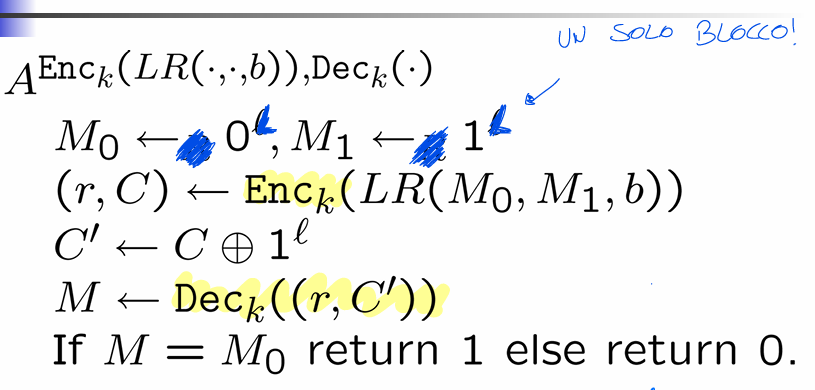
\includegraphics[width=0.5\linewidth]{Images/cifrari_simmetrici/attaccante_CPA_CTR.png}
\end{figure}
Durante queste operazioni, potremmo avere due flussi d'esecuzione:
\begin{enumerate}
    \item $(r,C) \xrightarrow{} C = F_k(r+1)\oplus 1^L$
    \item $(r,C) \xrightarrow{} C = F_k(r+1)\oplus 0^L = F_k(r+1)$ 
\end{enumerate}
E, al passo 3 avremo:
\begin{enumerate}
    \item $c \oplus 1^L = F_k(r+1)=F_k(r+1)\oplus 0^L$ Che rappresenta esattamente ciò che abbiamo al passaggio 2 di prima.
    \item $c \oplus 1^L = F_k(r+1)=F_k(r+1)\oplus 1^L$ che è esattamente ciò che abbiamo al passaggio 1 prima.
\end{enumerate}
Dunque, una volta effettuata la decifratura del messaggio, vedremo che in ogni caso se inviamo $M_1$ otteniamo $M_2$ e viceversa.
Notiamo che qualunque fosse stata la funzione di cifratura sottostante, non sarebbe cambiato nulla e ciò dimostra quanto gli attacchi CCA siano più forti rispetto agli attacchi CPA.
